\documentclass{article}
\usepackage[utf8]{inputenc}
\usepackage[spanish]{babel}
\usepackage{amsmath}
\usepackage{amssymb}
\usepackage{amsfonts}
\usepackage{hyperref}
\usepackage{textcomp}
\usepackage{graphicx}
\usepackage{pgfplots}
\usepackage{geometry}
\hypersetup{
    colorlinks=true,
    linkcolor=black,
    citecolor=green,
    filecolor=magenta,      
    urlcolor=cyan,
}
\geometry{
  top=3cm,            % Margen superior
  bottom=3cm,         % Margen inferior
  left=3cm,           % Margen izquierdo
  right=3cm           % Margen derecho
}

\title{Estadística 1}
\author{Jorge Miguel Alvarado Reyes}
\date{16 Agosto 2023}

\setlength{\parindent}{0pt}
\begin{document}

\begin{titlepage}
    \begin{center}
        
\includegraphics[width=0.2\textwidth]{../unam.png}
        \vspace*{.5cm}

        \LARGE
        \textbf{Universidad Nacional Autónoma de México}

        \vspace{0.5cm}
        \LARGE
        Facultad de Estudios Superiores Acatlán

        \vspace{2cm}

        \textbf{Apuntes} \\
        Optimizacion 2

        \vfill

        \vspace{1cm}

        \textbf{\large Autor:} \\
        Jorge Miguel Alvarado Reyes \\
        \vspace{.5cm}
        \normalsize \today

    \end{center}
\end{titlepage}
\newpage

\tableofcontents

\newpage

\section{29/01/2024}

\subsection{Evaluacion}

\begin{itemize}
    \item Parciales 50\% (2 examenes)
    \item Proyecto 50\%
    \item Participaciones: 1 pt extra
\end{itemize}

\subsection{Contacto}

877656@pcpuma.acatlan.unam.mx

\section{31/01/2023}

\subsection{Función Objetivo}
Maximizar (o Minimizar):
\begin{equation}
    Z = c_1x_1 + c_2x_2 + \cdots + c_nx_n
\end{equation}
donde $Z$ es la función objetivo y $c_i$ son los coeficientes de las variables de decisión $x_i$.

\subsection{Restricciones}
Sujeto a:
\begin{align}
    a_{11}x_1 + a_{12}x_2 + \cdots + a_{1n}x_n & \leq b_1         \\
    a_{21}x_1 + a_{22}x_2 + \cdots + a_{2n}x_n & \leq b_2         \\
                                               & \vdots \nonumber \\
    a_{m1}x_1 + a_{m2}x_2 + \cdots + a_{mn}x_n & \leq b_m
\end{align}

donde $a_{ij}$ son los coeficientes de las restricciones y $b_i$ son los términos constantes de las restricciones.

\subsection{Variables de Decisión}
Las variables de decisión son:
\begin{equation}
    x_1, x_2, \ldots, x_n \geq 0
\end{equation}

\subsection{Conjuntos Convexos}

\textbf{Definición:} Sea \( S \subseteq \mathbb{R}^n \), se dice que \( S \) es convexo si para cualesquiera \( x, y \in S \), el segmento de línea que los une está contenido en \( S \). Es decir, \( tx + (1-t)y \in S \) para todo \( t \in [0,1] \).

\textbf{Ejemplo de Conjuntos Convexos:}
\begin{itemize}
    \item \textit{El intervalo en la recta real}: En \( \mathbb{R} \), cualquier intervalo \([a, b]\) es un conjunto convexo. Esto se debe a que, para cualesquiera \( x, y \in [a, b] \) y \( t \in [0,1] \), la combinación \( tx + (1-t)y \) también pertenecerá a \([a, b]\).

    \item \textit{El espacio euclidiano \( \mathbb{R}^n \)}: Todo el espacio \( \mathbb{R}^n \) es un conjunto convexo, ya que cualquier segmento de línea entre dos puntos en \( \mathbb{R}^n \) también pertenece a \( \mathbb{R}^n \).

    \item \textit{Polihedros}

    \item \textit{Esferas}

    \item \textit{Elipsoides}

    \item \textit{Semiespacios}
\end{itemize}

\textbf{¿El vacio es convexo?}

En el caso del conjunto vacío, esta definición se cumple de manera un poco peculiar. Dado que no hay ningún par de puntos dentro del conjunto vacío (ya que no contiene puntos), no hay segmentos de línea que verificar. En términos lógicos, la afirmación de que "todos los segmentos de línea entre pares de puntos en \(\emptyset\) están contenidos en \(\emptyset\)" es verdadera por vacuidad; es decir, es verdadera porque no hay contraejemplos posibles dentro del conjunto vacío.

\vspace{.25cm}

\textbf{Demostración:}

Proposición: Sean \(S_1, S_2 \subseteq \mathbb{R}^n\), conjuntos convexos. Entonces, \(S_1 \cap S_2\) es convexo.

\begin{itemize}
    \item Si \(S_1 \cap S_2 = \emptyset\), entonces la afirmación se verifica, ya que el conjunto vacío es convexo.
    \item Si \(S_1 \cap S_2 \neq \emptyset\), sean \(x, y \in S_1 \cap S_2\). El segmento que une \(x\) y \(y\), denotado como \(\overline{xy}\), debe pertenecer tanto a \(S_1\) como a \(S_2\) puesto que ambos son conjuntos convexos. Por lo tanto, \(\overline{xy} \in S_1\) y \(\overline{xy} \in S_2\), lo que implica que \(\overline{xy} \in S_1 \cap S_2\). Esto demuestra que la intersección de dos conjuntos convexos es también convexa.
\end{itemize}

Consideremos los hemiespacios:
\[ H_t = \{(x, y) \in \mathbb{R}^2 \,|\, ax + by + c \leq 0\} \]
Aplicando la proposición anterior a los hemiespacios, concluimos que la intersección de dos hemiespacios es convexa. Geométricamente.

\vspace{.25cm}

\textbf{Definición:}

Un conjunto convexo y acotado se denomina \textit{politopo}. Si tal politopo se describe como la intersección de hemiespacios, en la terminología de programación lineal se le llama \textit{región de factibilidad}. El \textit{simplex} es un algoritmo que se basa en la búsqueda de soluciones óptimas explorando los "vértices" de dicha región.

\begin{equation}
    2x + 3y \leq 6
\end{equation}

\begin{align}
    x & \geq 0 \\
    y & \geq 0
\end{align}

\begin{center}
    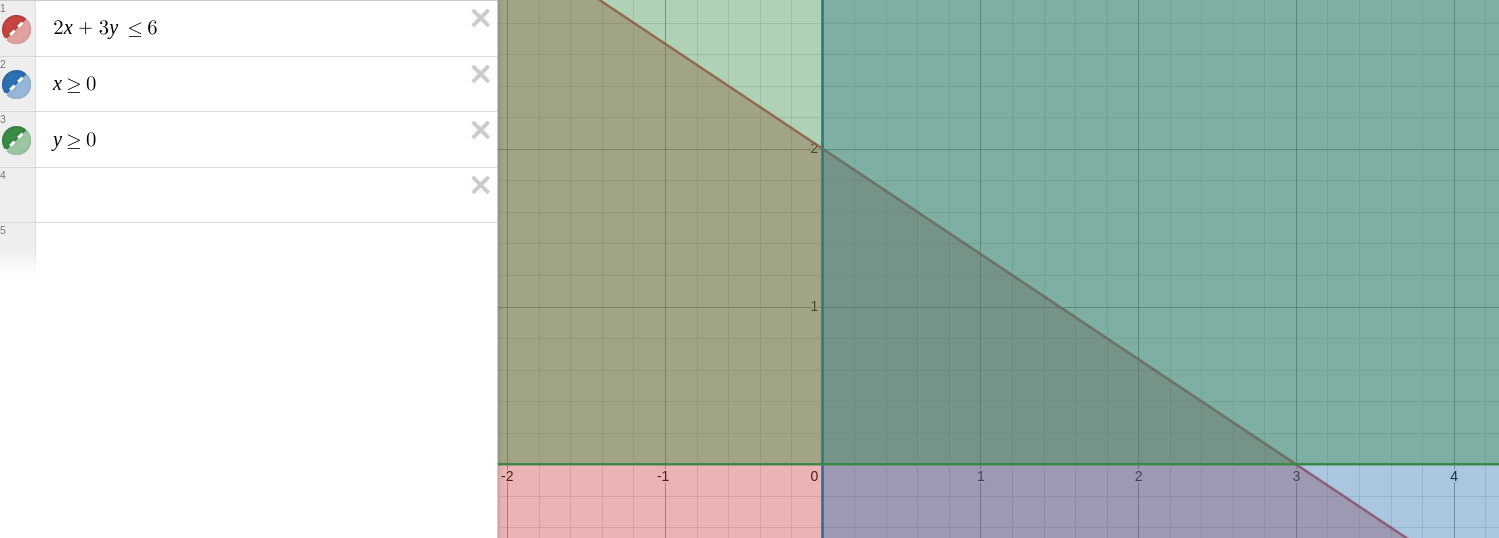
\includegraphics[width=0.7\textwidth]{./imagenes/imagen1.png}
\end{center}

El conjunto de funcionales lineales es un E.Vectorial, llamado el dual de $\mathbb{R}^n$, y se denota como $(\mathbb{R}^n)^*$
\newpage
\section{02/02/2024}

Maximizar la funcion

\begin{equation}
    Z = x_1 + x_2
\end{equation}

entre los vecotres $(x_1, x_2) \in \mathbb{R}$ sujetos a las restircciones:

\begin{align}
    x_2 + x_1  & \leq 1  \\
    x_1 + 6x_2 & \leq 15 \\
    4x_1 - x_2 & \leq 10
\end{align}

\begin{center}
    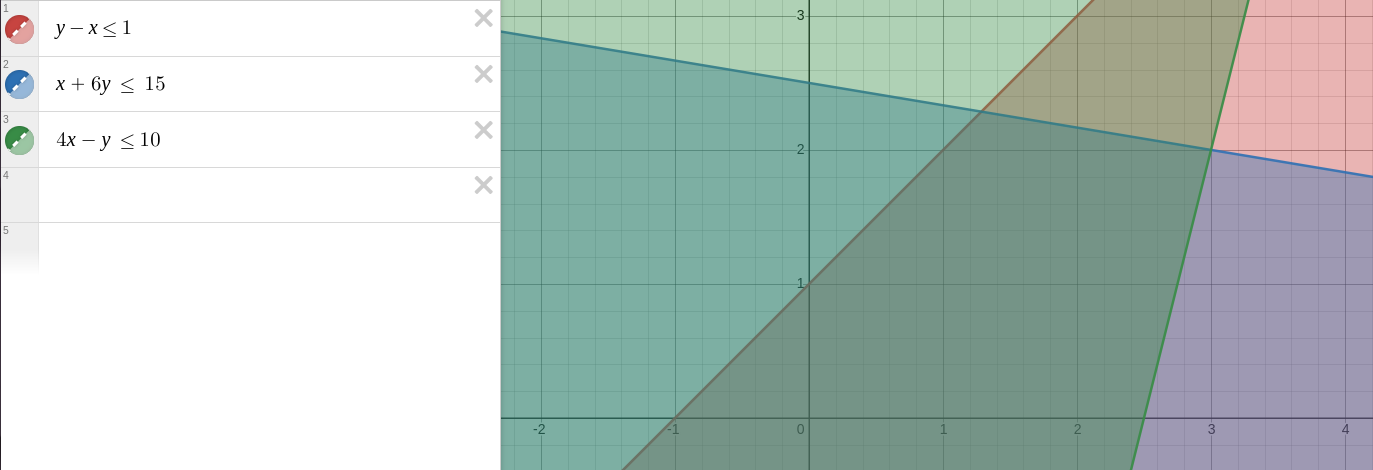
\includegraphics[width=0.7\textwidth]{./imagenes/imagen2.png}
\end{center}

\begin{enumerate}
    \item \textbf{Espacio Vectorial:} Un espacio vectorial es una colección de vectores, que pueden ser sumados entre sí y multiplicados por números, llamados escalares. Estos espacios son fundamentales en el álgebra lineal.
    \item \textbf{Subespacio Vectorial:} Un conjunto de vectores que forma un espacio vectorial por sí mismo dentro de un espacio vectorial más grande, cumpliendo con ciertas propiedades como contener el vector cero.
    \item \textbf{Base de Espacio Vectorial:} Un conjunto de vectores linealmente independientes en un espacio vectorial que abarcan el espacio completo, determinando su dimensión.
    \item \textbf{Rango de una Matriz:} La dimensión del espacio vectorial generado por las columnas o filas de una matriz, indicando el número máximo de columnas o filas linealmente independientes.
    \item \textbf{Transformaciones Lineales:} Funciones entre espacios vectoriales que respetan la adición de vectores y la multiplicación por escalares, fundamentales para entender el cambio entre diferentes espacios vectoriales.
    \item \textbf{Espacio Afín:} Generalización de los espacios vectoriales que permite sumas entre puntos y vectores sin un origen fijo, centrando en la dirección y distancia entre puntos.
\end{enumerate}
\newpage
\section{09/02/2024}

Maximizar \( z = x_1 + x_2 \)

Sujeto a:

\begin{align*}
    -x_1 + x_2 + x_3 & = 1 \\
    x_1 + x_4        & = 3 \\
    x_2 + x_5        & = 2 \\
\end{align*}

\section{15/03/2024}
\subsection*{Fase 1 - Encontrar una SBF inicial}

\begin{itemize}
    \item Esquina noroeste
    \item Costo mínimo
    \item Vogel
\end{itemize}

\subsection*{Fase 2 - Optimizar la solución encontrada en la fase 1}

\begin{itemize}
    \item Verificar si
          \[p + q - 1 = \text{Número de celdas marcadas}\]
\end{itemize}

Si no (caso degenerado), paso 2; si sí, paso 3.

2) Convertir las celdas no marcadas hasta validar \(p + q - 1 = \text{número de celdas}\). La elección de las variables no básicas es:

\begin{itemize}
    \item Elija la celda no marcada de costo mínimo.
    \item Si desde esta no existen caminos cerrados (circuitos), etiquétela asignándole un envío de E.
    \item De otra manera, intente con la siguiente celda de costo mínimo.
\end{itemize}

3) Condición de optimalidad

Evalue la factibilidad del dual para las variables básicas

\[u_i + v_j = c_{ij}\]

Para las variables no básicas

\[u_i + v_j \leq c_{ij}\]

Si se verifican, esta SBF es óptima. Presente conclusiones; sino, vaya al paso 4.

4) Entre las celdas que violan \(u_i + v_j \leq c_{ij}\), evalúe
\[|c_{ij} - u_i - v_j|\] y elija la de mayor valor.

5) (Pivote) Desde esta, trace un circuito asignando de manera alternada \(+ , -\) de modo que elija el mínimo entre los envíos de celdas negativas y sume esta cantidad a cada celda. Esto produce una nueva SBF.

6) Ejecute el paso 3.

\subsection*{Ejemplo}

La siguiente tabla representa un PT. encuentre una SBF inicial aplicando costo minimo y apartir de esta encuetre el optimo

\begin{tabular}{c|c|c|c|c|c|c}
            & $v_1$ & $v_2$ & $v_3$ & $v_4$ & $v_5$ & suministros \\ \hline
    $u_1$   & 10    & 2     & 3     & 15    & 9     & 35          \\ \hline
    $u_2$   & 5     & 10    & 15    & 2     & 4     & 40          \\ \hline
    $u_3$   & 15    & 5     & 14    & 7     & 15    & 20          \\ \hline
    $u_4$   & 20    & 15    & 13    & 25    & 8     & 30          \\ \hline
    Demanda & 20    & 20    & 40    & 10    & 35    & 125=125     \\
\end{tabular}


\section*{Palabras Clave}

\begin{itemize}
    \item Hemiespacios
    \item Politipos
    \item Espacios vectoriales
    \item Gradiente: Direccion de mayor crecimiento
\end{itemize}

\end{document}